\section{Experimentación}\label{sec:experimentacion}

En esta sección mostraremos los resultados de las pruebas con los distintos métodos de preprocesado de datos y modelos; con el objetivo de encontrar la combinación que nos dé los mejores resultados.

Antes de comentar específicamente los distintos métodos que probaremos, explicaremos la forma en la que se han realizado estas pruebas.
Como hemos comentado anteriormente, separamos los datos de entreno y prueba aplicando la opción de \textit{stratify} y con una proporción de \textit{75/25\%} respectivamente.

Una vez separados los conjuntos de datos, los tenemos que preprocesar. Para ello, hemos utilizado el objeto \textit{Pipeline} \cite{sklearnp32:online}, el cual nos permite encadenar diferentes pasos de preprocesado para entrenar diferentes modelos de forma sencilla. Por ejemplo, si queremos probar diferentes modelos, podemos hacerlo de la siguiente forma: 

\begin{enumerate}
    \item Instanciamos los objetos de las diferentes clases de preprocesado que queramos probar con sus respectivos valores. En el caso excepcional de la \textit{primera derivada}, hemos creado nuestro propio \textit{Transformer} (objeto de ``preprocesado'') que aplica la derivada a los datos.
    \item Los agregamos a la \textit{Pipeline} en orden.
    \item Ajustamos la \textit{Pipeline} sobre el conjunto de datos de entreno.
    \item Aplicamos la \textit{Pipeline} ya configurada sobre los datos de entreno y prueba. 
\end{enumerate}


El \textit{Pipeline} nos ofrece la ventaja de poder guardar y cargar tanto el orden del procedimiento, como la configuración de los pasos intermedios para aplicarlos más adelante de forma sencilla. Por ejemplo el \textit{StandardScaler}, para modificar los datos de forma que tengan media 0 y varianza 1, guarda la media y la varianza de cada columna para poder aplicarla más adelante.

Vale la pena comentar también que este objeto de \textit{Pipeline} nos ayuda a compartir la configuración del preprocesado entre la aplicación de entrenamiento de modelos y la de visualización de las predicciones sobre los archivos \gls{bil}.

Una vez hemos preprocesado los datos y entrenado los modelos; para evaluarlos, hemos utilizado la métrica \textit{Balanced Accuracy}, la cual hemos comentado en la \textit{Sección\ \ref{sec:metrics}}.

\subsection{Análisis del impacto de la primera derivada}

Para probar que, como hemos comentado antes, el aplicar la primera derivada sobre los datos nos puede ayudar a la hora de predecir, podemos comparar los resultados de entrenar con o sin derivar en la \textit{Tabla\ \ref{tab:nopreprocessing-derivative-results}}. En esta, podemos ver los resultados de entrenar la batería de modelos y su \textit{Balanced Accuracy} la cual ha mejorado un \textbf{1.481 (2.4\%)} respecto a no haber preprocesado los datos, por lo tanto, continuaremos aplicando la derivada en los siguientes pasos.

Además en la \textit{Tabla\ \ref{tab:nopreprocessing-derivative-results}} podemos ver un comportamiento que se repite, hay algunos modelos con un \textit{Balanced Accuracy} de $50$ (en nuestro caso es este valor, pues tenemos dos clases), lo cual nos indica que el modelo no ha sido capaz de predecir correctamente la clase minoritaria. Esto se debe a que los datos están desbalanceados y el modelo se aprovecha de ello, prediciendo siempre la clase mayoritaria.


\begin{table}[!ht]
    \centering
    \begin{tabular}{|c|c|c|}
        \hline
        & \textit{Derivative} & \textit{No preprocessing} \\ \hline
        Model Name & Balanced accuracy & Balanced accuracy \\ \hline
        XGBoost & 50 & 50 \\ 
        Stochastic Gradient Descent & 50 & 50 \\ 
        Random Forest & 66.531 & 70.069 \\ 
        Quadratic Discriminant Analysis & 50 & 50 \\ 
        Multi-Layer Perceptron & 51.114 & 50 \\ 
        Linear Discriminant Analysis & 53.96 & 54.306 \\ 
        LightGBM & 71.846 & 62.632 \\ 
        K-Neighbors & 71.289 & 82.46 \\ 
        Extra Trees & 78.756 & 76.438 \\ 
        Decision Tree & \textbf{67.224} & 50 \\ \hline
        \textit{Average} & \textbf{61.072} & 59.591 \\ \hline
    \end{tabular}
    \caption{Comparación de los resultados de entrenar utilizando la derivada y sin preprocesar. Fuente propia.}\ \label{tab:nopreprocessing-derivative-results}
\end{table}

\subsection{Análisis del impacto de aplicar la transformada}

Podemos ver los resultados de entrenar utilizando la transformada sobre los datos derivados en la \textit{Tabla\ \ref{tab:derivative-transformed-results}}, vemos que la métrica \textit{Balanced Accuracy} en general empeora en un \textbf{1.233 (-2.0\%)}, así que continuaremos las pruebas sin añadir la transformada al preprocesado.

\begin{table}[!h]
    \centering
    \begin{tabular}{|c|c|c|}
        \hline
            & \textit{Transformer \& derivative} & \textit{Derivative} \\ \hline
            Model Name & Balanced accuracy & Balanced accuracy \\ \hline
            XGBoost & 50 & 50 \\ 
            Stochastic Gradient Descent & 50 & 50 \\ 
            Random Forest & 66.531 & 66.531 \\ 
            Quadratic Discriminant Analysis & \textbf{55.149} & 50 \\ 
            Multi-Layer Perceptron & 50 & 51.114 \\ 
            Linear Discriminant Analysis & 52.529 & 53.96 \\ 
            LightGBM & 71.846 & 71.846 \\ 
            K-Neighbors & \textbf{56.143} & 71.289 \\ 
            Extra Trees & 78.967 & 78.756 \\ 
            Decision Tree & 67.224 & 67.224 \\ \hline
            \textit{Average} & 59.839 & \textbf{61.072} \\ \hline
    \end{tabular}
    \caption{Comparación de los resultados de entrenar transformando y derivando los datos; frente a solo derivando. Fuente propia.}\ \label{tab:derivative-transformed-results}
\end{table}

\subsection{Análisis del impacto de la estandarización de los datos}

Al aplicar la estandarización de los datos después de derivarlos obtenemos los resultados de la \textit{Tabla\ \ref{tab:derivative-standarization-results}}, los cuales en general son notablementes mejores que los anteriores, viendo una mejora del \textbf{3.014 (4.9\%)} en la \textit{Balanced Accuracy}. Estas mejoras ocurren en los modelos marcados en la tabla, \textit{QDA} y \textit{MLP}.


\begin{table}[!h]
    \centering
    \begin{tabular}{|c|c|c|}
        \hline
        & \textit{Derivative \& Scaler} & \textit{Derivative} \\ \hline
        Model Name & Balanced accuracy & Balanced accuracy \\ \hline
        XGBoost & 50 & 50 \\
        Stochastic Gradient Descent & 49.834 & 50 \\ 
        Random Forest & 66.531 & 66.531 \\ 
        Quadratic Discriminant Analysis & \textbf{72.358} & 50 \\ 
        Multi-Layer Perceptron & \textbf{59.41} & 51.114 \\ 
        Linear Discriminant Analysis & 53.96 & 53.96 \\ 
        LightGBM & 71.981 & 71.846 \\ 
        K-Neighbors & 70.807 & 71.289 \\ 
        Extra Trees & 78.756 & 78.756 \\ 
        Decision Tree & 67.224 & 67.224 \\ \hline
        \textit{Average} & \textbf{64.086} & 61.072 \\ \hline
    \end{tabular}
    \caption{Comparación de los resultados de entrenar derivando y estandarizando los datos; frente a solo derivando. Fuente propia.}\ \label{tab:derivative-standarization-results}
\end{table}


\subsection{Impacto del aumento y disminución de dimensionalidad de los datos}


Por último, aun siendo un paso generalmente recomendado, el aumento y disminución de dimensionalidad nos ha dado los resultados de la \textit{Tabla\ \ref{tab:derivative-standarization-dimensionality-results}}, los cuales son significativamente peores que los anteriores empeorando la \textit{Balanced Accuracy} en un \textbf{5.526 (-8.6\%)}. Por lo tanto, continuaremos con los datos derivados y estandarizados sin aumentar o disminuir la dimensionalidad de los datos.

\begin{table}[!h]
    \centering
    \resizebox{\textwidth}{!}{\begin{tabular}{|c|c|c|}
        \hline
        & \textit{Derivative \& Scaler \& Polynomial Features \& PCA} & \textit{Derivative \& Scaler} \\ \hline
        Model Name & Balanced accuracy & Balanced accuracy \\ \hline
        XGBoost & 50 & 50 \\ 
        Stochastic Gradient Descent & 52.439 & 49.834 \\ 
        Random Forest & 61.939 & 66.531 \\ 
        Quadratic Discriminant Analysis & {63.234} & {72.358} \\ 
        Multi-Layer Perceptron & 54.682 & 59.41 \\ 
        Linear Discriminant Analysis & 50.903 & 53.96 \\ 
        LightGBM & {62.933} & {71.981} \\ 
        K-Neighbors & {64.092} & {70.807} \\ 
        Extra Trees & 70.37 & 78.756 \\ 
        Decision Tree & 55.014 & 67.224 \\ \hline
        \textit{Average} & \textbf{58.560} & \textbf{64.086} \\ \hline
    \end{tabular}}
    \caption{Comparación de los resultados de entrenar derivando, estandarizando y ajustando la dimensionalidad de los datos; frente a solo derivando y estandarizando. Fuente propia.}\ \label{tab:derivative-standarization-dimensionality-results}
\end{table}


\subsection{Selección de modelos y \textit{hyperparameter tuning}}\ \label{sec:entrenamiento}

Una vez encontrada una combinación de pasos de preprocesado que nos mejora los resultados, podemos pasar al siguiente paso de selección de los modelos. Habiendo entrenado ya los modelos, vemos en la \textit{Tabla\ \ref{tab:final-training-results}} que algunos hacen \textit{overfitting}. El \textit{overfitting} ocurre cuando un modelo se ajusta demasiado a los datos con los que ha entrenado y no generaliza bien, es decir que predice mejor los datos con los que ha entrenado que datos nuevos. Esto lo podemos ver en la tabla comparando los valores de las columnas \textit{Train} y \textit{Test score}.

Donde lo podemos ver más claramente es en \textit{KNeighbors}, vemos en la \textit{Figura\ \ref{fig:lc-knn}} que, para cualquier cantidad de datos con los que entrenemos el modelo, siempre predecirá bien con los que ha entrenado y no tanto con los demás. Nuestro objetivo es intentar que ambos valores no sean tan dispares y que sean lo más altos posibles, para ello aplicaremos \textit{hyperparameter tuning}.

\begin{table}[!ht]
    \centering
    \begin{tabular}{|c|ccc|}
    \hline
        Model Name & Train score & Test score & Balanced accuracy \\ \hline
        XGBoost & 82 & 82 & 50 \\ 
        Stochastic Gradient Descent & 64.815 & 56.444 & 49.834 \\ 
        Random Forest & \textbf{99.926} & \textbf{87.778} & 66.531 \\ 
        Quadratic Discriminant Analysis & \textbf{96.148} & \textbf{83.111} & 72.358 \\ 
        Multi-Layer Perceptron & 90.815 & 84 & 59.41 \\ 
        Linear Discriminant Analysis & \textbf{85.333} & \textbf{78.222} & 53.96 \\ 
        LightGBM & 82.222 & 72.222 & 71.981 \\ 
        K-Neighbors & \textbf{100} & \textbf{86.889} & 70.807 \\ 
        Extra Trees & \textbf{99.63} & \textbf{90.444} & 78.756 \\ 
        Decision Tree & 56.963 & 58.889 & 67.224 \\
    \hline
    \end{tabular}
    \caption{Tabla ampliada de los resultados de entrenar los modelos utilizando la derivada y \textit{StandardScaler}. Fuente propia.}\ \label{tab:final-training-results}
\end{table}

\begin{figure}[!h]
    \centering
    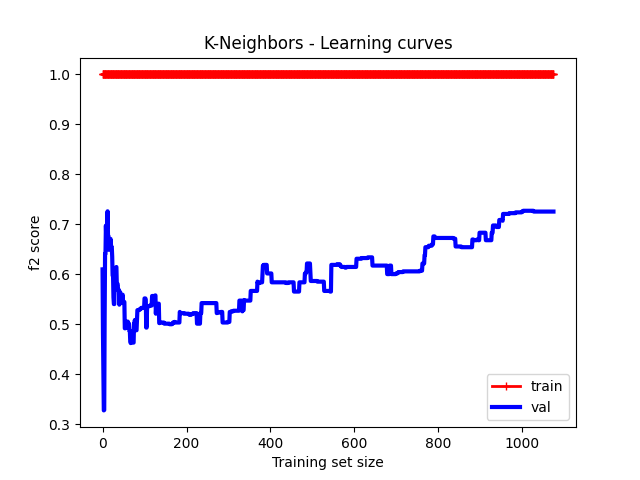
\includegraphics[width=0.7\linewidth]{media/images/learing-curves-knn.png}
    \caption{Gráfico de la curva de aprendizaje del modelo \textit{K-Neighbors} entrenándolo y probándolo sobre los datos de entreno únicamente. Fuente propia}\ \label{fig:lc-knn}
\end{figure}

El \textit{hyperparameter tuning} tiene como objetivo encontrar un conjunto de parámetros que maximice el rendimiento del modelo sobre los datos de prueba. En nuestro caso, como los datos están desbalanceados, podemos utilizar como función a optimizar el \textit{Balanced Accuracy}. Como cada modelo es distinto, debemos encontrar los parámetros adecuados para cada uno. 

Como no todos los modelos nos han dado buenos resultados y el \textit{hyperparameter tuning} es un proceso costoso, para ahorrarnos tiempo podemos utilizar solamente los mejores, como hemos visto en la \textit{Tabla\ \ref{tab:final-training-results}} hay modelos que tienen mejores resultados que otros. Así que escogeremos los cuatro con mejor \textit{balanced accuracy}, es decir: \textit{Extra Trees, Quadratic Discriminant Analysis, LightGBM y K-Neighbors}.

Realizaremos el \textit{hyperparameter tuning} en dos pasos, primeramente utilizaremos \textit{Random Search} y después \textit{Grid Search}, ya implementados en \textit{sklearn}.
Ambos métodos utilizan \textit{cross-validation}, una técnica para evitar el \textit{overfitting} (y el \textit{underfitting}) que consiste en la división de los datos de entreno en partes iguales. \cite{31Crossv20:online}

Una vez divididos los datos de entreno en \textit{N} partes, se itera sobre cada una de ellas, utilizando \textit{N-1} partes para entrenar el modelo y la restante para evaluarlo. Una vez obtenemos los modelos entrenados sobre las diferentes partes, los comparamos con la función de rendimiento que queramos optimizar y seleccionamos el mejor. Una vez seleccionado el mejor modelo, lo probamos sobre los datos de prueba y obtenemos los resultados finales. Podemos ver este proceso gráficamente en la \textit{Figura\ \ref{fig:cross-validation}}.

\begin{figure}[!h]
    \centering
    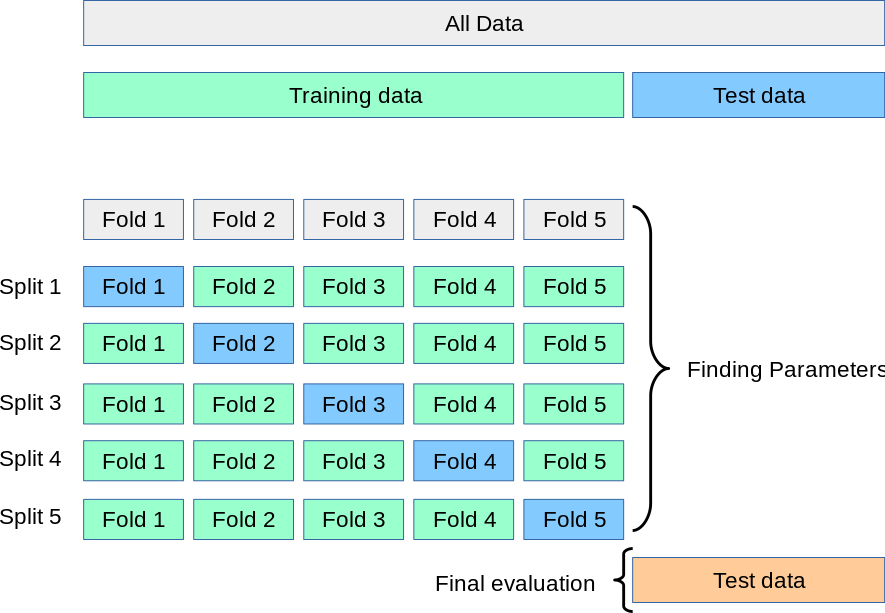
\includegraphics[width=0.7\linewidth]{media/images/cross-validation.png}
    \caption{\textit{Cross-validation} explicado gráficamente. Fuente:\ \cite{31Crossv20:online}}\ \label{fig:cross-validation}
\end{figure}


El \textit{random search} consiste en la búsqueda de estos parámetros habiendo definido un rango de posibilidades. Es decir, para cada parámetro que le queramos pasar al modelo definiremos un rango de valores que puede tener, entonces el \textit{random search} entrena el modelo repetidas veces con una permutación aleatoria de sus parámetros y se guarda los resultados. Podemos ver un ejemplo en el \textit{Código\ \ref{code:random-search-example}}.
Podemos ir probando diferentes parámetros y rangos hasta que estemos satisfechos con el resultado.


Una vez estemos contentos con los resultados, los refinaremos utilizando \textit{grid search}. A diferencia del \textit{random search}, el \textit{grid search} prueba todas las posibles combinaciones que le pasemos como parámetro y, consecuentemente, es mucho más lento. Por ello, utilizaremos el \textit{grid search} con los valores de los parámetros que dan los cinco mejores resultados del paso anterior, los cuales son potencialmente un máximo local. Una vez definido un rango de parámetros para cada modelo seleccionado, obtenemos los resultados de la \textit{Tabla\ \ref{tab:hyperparameter-tuning-results}} donde vemos que los resultados del \textit{Random Search} y los de \textit{Grid Search} son iguales, salvo por \textit{Extra Trees}, en el cual el hacer \textit{Grid Search} sí que nos aporta mejores resultados. En general, vemos que hemos obtenido resultados parecidos a los de los modelos sin refinar, salvo por \textit{K-Neighbors}, que ha mejorado en un \textbf{19.467 (27.5\%)}, y \textit{Extra Trees}, que ha empeorado en un \textbf{12.586 (-16.0\%)}.
Por lo tanto, deberíamos ajustar el rango de los parámetros que les pasamos a los modelos que no han dado buenos resultados y volver a entrenarlos hasta que estemos satisfechos. En nuestro caso no lo haremos, sino que retrocederemos unos pasos y probaremos otras técnicas.

\begin{table}[!h]
    \centering
    \resizebox{\textwidth}{!}{\begin{tabular}{|c|ccc|}
        \hline
        Model name & Train score & Test score & Balanced accuracy \\ \hline
        RS K-Neighbors & 100 & 90.274 & 90.274 \\ 
        GS K-Neighbors & 100 & 90.274 & 90.274 \\ 
        RS Quadratic Discriminant Analysis & 97.491 & 72.358 & 72.358 \\ 
        GS Quadratic Discriminant Analysis & 97.491 & 72.358 & 72.358 \\ 
        RS LightGBM & 86.013 & 71.018 & 71.018 \\ 
        GS LightGBM & 86.013 & 71.018 & 71.018 \\ 
        GS Extra Trees & 82.957 & 66.17 & 66.17 \\ 
        RS Extra Trees & 69.492 & 65.854 & 65.854 \\ \hline
        \end{tabular}}
    \caption{Resultados del primer entrenamiento con hyperparameter tuning. Fuente propia.}\ \label{tab:hyperparameter-tuning-results}
\end{table}
\clearpage

\subsection{Balanceo de datos}\ \label{sec:i2-balance}

Como hemos comentado en la \textit{Sección\ \ref{sec:balance}}, los datos están desbalanceados, por lo tanto, podemos aplicar diferentes técnicas para balancearlos. En nuestro caso, hemos probado dos técnicas, \textit{undersampling} y \textit{oversampling}.

\subsubsection{\textit{Undersampling}}

Al probar los algoritmos mencionados en la \textit{Sección\ \ref{sec:undersampling}}, obtenemos los resultados de la \textit{Tabla\ \ref{tab:undersampling-methods}}, en la cual hemos agregado una columna, \textit{Avg. score diff}, que nos indica la diferencia entre el \textit{Train} y \textit{Test score} para compararlos mejor, pues las \textit{Balanced Accuracy} dan resultados bastante parecidos. Esta ``nueva'' métrica nos indica cuánto \textit{overfitting} hacen los modelos que se entrenan sobre el dataset generado, por lo tanto, cuanto más cercana a \textit{0} sea, mejor. Podemos ver que, en general, los diferentes \textit{Near Miss}, obtienen resultados bastante peores que los otros métodos. En cuanto a los otros tres algoritmos restantes, podemos ver que el \textit{Tomek Links} es el único que tiene mejores resultados que el \textit{dataset} sin hacer \textit{undersampling}, por lo tanto, continuaremos con este método.

\begin{table}[!h]
    \centering
    \begin{tabular}{|c|cc|} \hline
        & Avg. score diff & Avg. Balanced Accuracy \\ \hline
        \textit{\textbf{Baseline: No undersampling}} & 8.202 & 63.665 \\ 
        \textit{\textbf{Tomek Links}} & 7.972 & 64.739 \\ 
        \textit{Edited Nearest Neighbours (mode)} & 8.641 & 64.416 \\ 
        \textit{Random UnderSampler} & 9.176 & 63.656 \\ 
        \textit{Near Miss v3} & 9.548 & 62.359 \\ 
        \textit{Edited Nearest Neighbours (all)} & 10.132 & 66.405 \\ 
        \textit{Near Miss v1} & 35.903 & 62.632 \\ 
        \textit{Near Miss v2} & 42.761 & 61.150 \\ \hline
    \end{tabular}
    \caption{Resumen de los resultados de entrenar los modelos básicos sobre el \textit{dataset} reducido con los diferentes métodos de \textit{undersampling}. Fuente: propia.}\ \label{tab:undersampling-methods}
\end{table}

Una vez hemos aplicado \textit{Tomek Links} sobre el \textit{dataset}, nos quedamos con el número de muestras de la \textit{Tabla\ \ref{tab:balance-tl-comparison}}, en la cual podemos ver que tan solo se han eliminado \textbf{$12$} y aun así han habido algunas mejoras.

\begin{table}[!h]
    \centering
    \begin{tabular}{|c|cc|} \hline
        & Good samples & Bad samples \\ \hline
        Before undersampling & 1107 & 243 \\
        After undersampling & 1095 & 243 \\ \hline
    \end{tabular}
    \caption{Comparación de las muestras antes y después de aplicar \textit{Tomek Links}. Fuente propia.}\ \label{tab:balance-tl-comparison}
\end{table}

\begin{table}[!h]
    \centering
    \begin{tabular}{|c|ccc|}
    \hline
        Model Name & Train score & Test score & Balanced accuracy \\ \hline
        XGBoost & 81.839 & 82 & 50 \\ 
        Stochastic Gradient Descent & 65.845 & 57.111 & 54.095 \\ 
        Random Forest & 100 & 86.444 & 63.791 \\ 
        \textbf{Quadratic Discriminant Analysis} & 96.487 & 83.778 & 72.282 \\ 
        Multi-Layer Perceptron & 90.284 & 82.889 & 60.659 \\ 
        Linear Discriminant Analysis & 85.202 & 77.778 & 54.17 \\ 
        \textbf{LightGBM} & 83.857 & 73.333 & 73.141 \\ 
        \textbf{K-Neighbors} & 100 & 87.111 & 71.424 \\ 
        \textbf{Extra Trees} & 99.552 & 91.111 & 80.608 \\ 
        Decision Tree & 57.1 & 58.889 & 67.224 \\ \hline
        \textit{Average} & 86.017 & 78.044 & 64.739 \\ \hline
    \end{tabular}
    \caption{Resultados de entrenar los modelos básicos habiendo balanceado el \textit{dataset} utilizando el método \textit{Tomek Links}. Fuente propia.}\ \label{tab:tomeklinks-basic-training}
\end{table}

\clearpage
\subsubsection{\textit{Oversampling}}

Para balancear el \textit{dataset}, como hemos comentado en la \textit{Sección\ \ref{sec:oversampling}}, hemos utilizado los sintetizadores de la librería \textit{SDV} para generar datos sintéticos. Además de los sintetizadores, la librería nos ofrece métodos para evaluar la calidad de los datos generados en forma de \textit{quality reports}. Estos \textit{quality reports} contienen la similitud estadística de los datos generados con los datos reales.

Una vez entrenados los sintetizadores y generados los datos, obtenemos los resultados de la \textit{Tabla\ \ref{tab:oversampling-quality-report}}, en los cuales podemos ver que la calidad de los datos generados por el sintetizador \textit{Gaussian Copula Synthesizer} son mejores.

\begin{table}[!h]
    \centering
    \resizebox{0.8\linewidth}{!}{\begin{tabular}{|c|ccc|} \hline
        Synthesizer & Column Shapes & Column Pair Trends & Overall Quality \\ \hline
        Gaussian Copula Synthesizer & 94.75 & 99.83 & 97.29 \\
        TVAE Synthesizer & 84.37 & 74.97 & 79.64 \\ \hline
    \end{tabular}}
    \caption{Resultados del \textit{quality report} de los datos generados con los sintetizadores. Fuente propia}\ \label{tab:oversampling-quality-report}
\end{table}

Una vez tenemos los sintetizadores entrenados sobre la clase minoritaria, generamos nuevos datos y los añadimos al \textit{dataset} original, entrenamos los modelos básicos y obtenemos los resultados de la \textit{Tabla\ \ref{tab:balanced-basic-training}} donde podemos ver que, en general, los modelos resultantes son peores que los que se han entrenado con datos que no utilizan ningún sintetizador (como los de la \textit{Tabla\ \ref{tab:tomeklinks-basic-training}}). Por lo tanto, a continuación mantendremos el paso de \textit{undersampling}, pero no utilizaremos \textit{oversampling}.

\begin{table}[!h]
    \centering
    \begin{tabular}{|c|ccc|}\hline
        Model Name & Train score & Test score & Balanced accuracy \\ \hline
        XGBoost & 90.411 & 80.667 & 53.523 \\
        Stochastic Gradient Descent & 85.571 & 71.111 & 53.96 \\
        Random Forest & 95.388 & 82.222 & 58.808 \\
        Quadratic Discriminant Analysis & 93.881 & 82.222 & 52.063 \\
        Multi-Layer Perceptron & 94.247 & 82.222 & 65.553 \\
        Linear Discriminant Analysis & 88.584 & 79.333 & 52.71 \\
        LightGBM & 90.868 & 80.667 & 53.041 \\
        K-Neighbors & 100 & 87.778 & 74.721 \\
        Extra Trees & 90.183 & 82.889 & 54.396 \\
        Decision Tree & 86.256 & 80.444 & 51.46 \\ \hline
        \textit{Average} & 91.539 & 80.956 & \textbf{57.024} \\ \hline
    \end{tabular}
    \caption{Resultados de entrenar los modelos básicos habiendo balanceado el \textit{dataset} con \textit{Tomek Links} y \textit{Gaussian Copula Synthesizer}. Fuente propia.}\ \label{tab:balanced-basic-training}
\end{table}

\subsection{Modelos \textit{ensemble}}

Vemos que los resultados del balanceo del \textit{dataset} comparados con el \textit{dataset} sin balancear de la \textit{Tabla\ \ref{tab:undersampling-methods}} han mejorado la calidad de los modelos en un \textbf{$1.074$ (1.7\%)} y también el \textit{overfitting} en un \textbf{$0.23$ (2.8\%)}. Para intentar mejorar aún más el \textit{overfitting} manteniendo la calidad de los modelos, podemos probar a utilizar modelos \textit{ensemble}. Este tipo de modelos consiste en la combinación de varias predicciones de diferentes modelos para obtener una predicción final. Creemos que no tiene mucho sentido hacer \textit{ensemble} del modelo \textit{Random Forest}, pues en sí ya es un modelo que hace \textit{ensemble}, pero para mantener la cohesión del trabajo lo incluiremos en los experimentos.

Nos centraremos en dos de ellos implementados en \textit{sklearn}: \textit{Voting Classifier} y \textit{Bagging Classifier}.
El primero, \textit{Voting Classifier}, entrena los modelos que lo componen sobre el \textit{dataset} y, a la hora de predecir, extrapola su predicción en base a las predicciones de estos modelos. Es decir, realiza una votación y la clase que más se vote es la que sale como predicción como podemos ver en la \textit{Figura\ \ref{fig:voting-classifiers}}. Hay dos tipos de votación, \textit{hard} y \textit{soft}. \textit{Hard} utiliza la clase mayormente predicha por los modelos, mientras que \textit{soft} tiene en cuenta la ``confianza'' de las predicciones. Es decir, no solo utiliza la clase predicha, sino que usa la probabilidad de cada clase a predecir a modo de peso. \cite{Ensemble96:online}

\begin{figure}[!h]
    \centering
    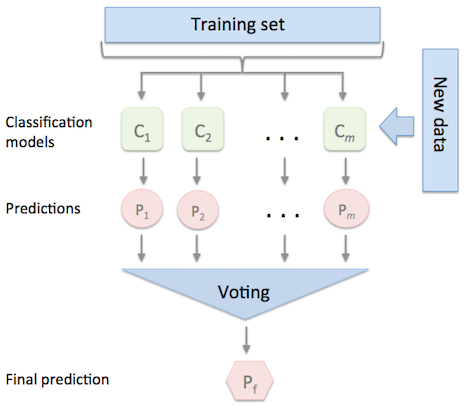
\includegraphics[width=0.7\linewidth]{media/images/majority_voting.png}
    \caption{Explicación gráfica del proceso de entreno y predicción de un \textit{Voting Classifier}. Fuente \cite{Ensemble96:online}.}\ \label{fig:voting-classifiers}
\end{figure}

Por otro lado el \textit{Bagging Classifier} entrena el mismo modelo sobre un subconjunto aleatorio del \textit{dataset} y luego agrega los resultados de las predicciones, ya sea haciendo la media o realizando una votación, para obtener una predicción final.\ \cite{sklearne53:online}

Antes de entrenar estos modelos, hemos de decidir qué otros modelos los compondran, por lo tanto, escogeremos los que han tenido mejores resultados al entrenarlos sobre el \textit{dataset} balanceado. Estos son los que mejores resultados tienen en la \textit{Tabla\ \ref{tab:tomeklinks-basic-training}}, es decir, \textit{K-Neighbors}, \textit{Quadratic Discriminant Analysis}, \textit{LightGBM} y \textit{Extra Trees}.


Primero entrenaremos los modelos \textit{Voting} para comparar los resultados de utilizar los diferentes tipos de votación \textit{soft} y \textit{hard}. Vemos en la \textit{Tabla\ \ref{tab:voting-results}} que el mejor modelo es el que combina \textit{Extra Trees} y \textit{LightGBM} utilizando la votación \textit{soft}, y en general, aunque la votación \textit{hard} tiende a tener menos \textit{overfitting}, la \textit{soft} obtiene mejores modelos, lo cual es curioso porque en la documentación \cite{Ensemble96:online} recomendaban utilizar \textit{hard} si los modelos componentes no estaban calibrados.

Para los modelos \textit{Bagging} vemos en la \textit{Tabla\ \ref{tab:bagging-results}} que el mejor modelo es el que utiliza \textit{Quadratic Discriminant Analysis}, aunque en general los modelos resultantes son peores que los de los \textit{Voting Classifiers} y que los modelos básicos. Esto podría ser debido a la baja cantidad de datos con los que se entrenan, pues al tener pocos datos de base y al hacer \textit{Bagging}, se generan subconjuntos de datos más pequeños, lo cual ayuda a no hacer \textit{overfitting} --- de hecho, podemos ver que el modelo que utiliza \textit{LGBM} tiene un \textit{Score diff.} negativo, lo que significa que es más preciso sobre los datos de prueba que los de entreno --- pero afecta a la calidad de los modelos resultantes.

\begin{table}[!h]
    \centering
    \resizebox{\textwidth}{!}{\begin{tabular}{|c|cc|cc|}
        \hline
        & \multicolumn{2}{|c|}{\textit{Soft voting}} & \multicolumn{2}{|c|}{\textit{Hard voting}} \\ \hline
        Estimators Name & Score diff. & Balanced accuracy & Score diff. & Balanced accuracy \\ \hline
        \textit{QDA \& LGBM} & 12.34 & 73.035 & 11.673 & 69.587 \\ 
        \textit{QDA \& KNN} & 13.023 & 72.267 & 9.871 & 60.373 \\ 
        \textit{QDA \& ET \& LGBM \& KNN} & 12.369 & 69.286 & 8.54 & 60.358 \\ 
        \textit{QDA \& ET} & 12.667 & 74.45 & 11.258 & 69.482 \\ 
        \textit{LGBM \& KNN} & 10.013 & 65.131 & 8.895 & 61.548 \\ 
        \textbf{\textit{ET \& LGBM}} & \textbf{7.778} & \textbf{80.322} & 8.134 & 73.803 \\ 
        \textit{ET \& KNN} & 12.444 & 69.286 & 8.096 & 62.556 \\ \hline
        \textit{Average} & 11.519 & 71.968 & 9.495 & 65.387\\ \hline
    \end{tabular}}
    \caption{Comparación de los resultados de entrenar los diferentes \textit{Voting Classifiers} sobre el \textit{dataset} balanceado utilizando los diferentes tipos de votación. Fuente propia.}\ \label{tab:voting-results}
\end{table}

\begin{table}[!h]
    \centering
    \begin{tabular}{|c|cc|}
        \hline
        Estimators name & Score diff. & Balanced accuracy \\ \hline
        \textit{QDA} & 8.918 & 69.783 \\ 
        \textit{LGBM} & -0.161 & 50.0 \\ 
        \textit{KNN} & 5.552 & 67.721 \\ 
        \textit{ET} & 11.402 & 67.148 \\ \hline
        \textit{Average} & 6.428 & 63.663 \\ \hline
    \end{tabular}
    \caption{Resultados de entrenar los diferentes \textit{Bagging Classifiers} sobre el \textit{dataset} balanceado. Fuente propia.}\ \label{tab:bagging-results}
\end{table}

\clearpage
\subsection{Hyperparameter tuning}\ \label{sec:hyperparameter-tuning-2}

Además de los nuevos modelos, podemos volver a probar a hacer \textit{hyperparameter tuning} sobre el dataset balanceado, obteniendo los resultados de la \textit{Tabla\ \ref{tab:hyperparameter-tuning-results-v2}} que son muy parecidos a los resultados del anterior \textit{hyperparameter tuning} (en la \textit{Tabla\ \ref{tab:hyperparameter-tuning-results}}), sin embargo, hemos encontrado una combinación de parámetros para el \textit{K-Neighbors} que da resultados algo mejores, siendo el mejor modelo (y combinación de pasos de preprocesado) que hemos encontrado hasta ahora.

\begin{table}[!h]
    \centering
    \begin{tabular}{|c|ccc|} \hline
        Model name & Train score & Test score & Balanced accuracy \\ \hline
        RS K-Neighbors & 100 & 91.509 & 91.509 \\ 
        GS K-Neighbors & 100 & 91.509 & 91.509 \\ 
        RS Quadratic Discriminant Analysis & 97.694 & 72.282 & 72.282 \\ 
        GS Quadratic Discriminant Analysis & 97.694 & 72.282 & 72.282 \\ 
        GS LightGBM & 85.107 & 71.304 & 71.304 \\ 
        RS LightGBM & 85.748 & 69.798 & 69.798 \\ 
        RS Extra Trees & 50 & 50 & 50 \\ 
        GS Extra Trees & 50 & 50 & 50 \\ \hline
    \end{tabular}
    \caption{Resultado del \textit{hyperparameter tuning} con el \textit{dataset} balanceado. Fuente propia.}\ \label{tab:hyperparameter-tuning-results-v2}
\end{table}